% Drawing 87/01-2 -- folder 87, batch 01, archive page 9 (PDF page 10).
% Transcription: dans la marge gauche, un croquis : une bande entre deux droites parallèles, un point marqué sur l'une, et une ligne brisée en zigzag entre les deux
% Kind: strip between two parallel lines with a zigzag. Method 2 (schematic redraw from the facsimile). Status: ok.
% Notes: Two nearly parallel lines bounding a strip, a marked point on the upper one (left end) with a tick to the right; from the point a broken zigzag line runs between the two lines (shape approximate).
% Coordinates: 1 unit = 1 mm = 1/100 of the crop width (bbox in page fractions: [0.14, 0.14, 0.36, 0.24]).
% Redrawn by Claude (claude-opus-5-5), issue #73, 2026-11-07; not checked by a human; not compiled (no TeX in the session).
% Rights: reproduces part of the work -- behind RENDER_TRANSCRIPTS, never published by itself.
\documentclass[tikz,border=3pt]{standalone}
\usepackage{amsmath,amssymb}
\usetikzlibrary{patterns,arrows.meta}
\tikzset{pencil/.style={black!45}, struck/.style={black!35}, mark/.style={circle,draw,inner sep=1.3pt}, pt/.style={circle,fill,inner sep=0.9pt}, opt/.style={circle,draw,fill=white,inner sep=1.1pt}}
\begin{document}
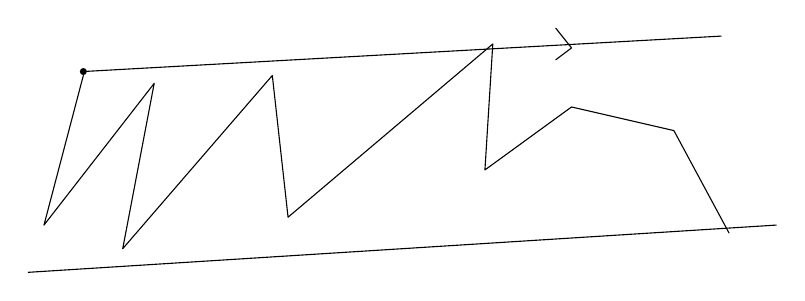
\begin{tikzpicture}[x=1mm,y=1mm,line cap=round,line join=round,font=\scriptsize]
\draw (11,-22.5) -- (92,-18);
\draw (4,-48) -- (99,-42);
\node[pt] at (11,-22.5) {};
\draw (71,-17) -- (73,-19.5) -- (71,-21);
\draw (11,-23) -- (6,-42) -- (20,-24) -- (16,-45) -- (35,-23) -- (37,-41) -- (63,-19) -- (62,-35) -- (73,-27) -- (86,-30) -- (93,-43);
\end{tikzpicture}
\end{document}
